\documentclass[letterpaper]{scrartcl}

\author{William Brown (whb2107)}

\usepackage{amsmath,amssymb,appendix,color,etoolbox,
  graphicx,index,listings,lscape,natbib,url}

\definecolor{gray}{gray}{0.95}

\renewcommand{\familydefault}{\sfdefault}

\lstset{
  language=Python,
  basicstyle=\footnotesize\ttfamily,
  numbersep=5pt,              
  tabsize=2,                  
  extendedchars=true,         
  breaklines=true,            
  stringstyle=\ttfamily, 
  showspaces=false,      
  showtabs=false,        
  xleftmargin=17pt,
  framexleftmargin=17pt,
  framexrightmargin=5pt,
  framexbottommargin=4pt,
  backgroundcolor=\color{gray},
  showstringspaces=false 
 }

\newcommand\imgfig[4]{
\begin{figure}[h]
  \centering
  \includegraphics[scale=#2]{figures/#1}
  \caption{#3}
  \label{fig:#4}
\end{figure}}

\newcommand\figref[1]{Figure \ref{fig:#1}}
\newcommand\tabref[1]{Table \ref{tab:#1}}
\newcommand\code[1]{\texttt{#1}}
\newcommand\pipe[0]{\;|\;}
\newcommand\st[0]{\;\mathrm{s.t.}\;}

\newindex{todo}{tod}{tnd}{TODO List}

\newcommand\todo[1]{
  % Add to todo list
  \index[todo]{#1}
  % Make the margin par
  \marginpar{
    \raggedright
    \textbf{TODO}:\\
    #1
  }
}

\newcommand\todolist{\printindex[todo]}

\setcounter{secnumdepth}{5}
\setcounter{tocdepth}{5}

\newcommand\startappendix{\appendix\appendixpage\addappheadtotoc}


\author{Benjamin Bardin \and William Brown 
  \and Dr. Paul Blaer}
\title{Stable Quadricopter Flight and 
  Telepresence using the Android Platform}

\begin{document}
\maketitle
\tableofcontents
\newpage

\todolist
\newpage

\section{Motivation}
\subsection{Objectives}
When we started this project, we had many different use cases for the
helicopter -- automatic target tracking, panaroma creation from the
video stream, even getting it to bring forgotten homework assignments
from our apartment to class. However, for the first iteration of both
the hardware and the software, we set our sights on more
immediately-acheivable goals: telepresence and stable flight
control. For telepresence, we wanted to be able to visualize the
Android device's location, orientation, acceleration and velocity in
real-time, as well as receive a video stream that compensated for
network latency and low bandwidth. For stable flight control, we
wanted a system that could maintain a hovering state within a narrow
radius of a given point (our target radius was ten feet) and could
respond to commands sent from a host computer.

\subsection{Progress}
\todo{Add progress once we know how much progress we've made}

\subsection{Future Goals}
The first goal is to acheive stable hovering. This will require a fair
amount of debugging, considering how much of our stability and
navigation software remains untested in the field, as well as manual
tuning of PID values (as will be discussed in section
\ref{sec:pilot}), which will no doubt be a lengthy process.

We have also discussed various uses of the helicopter platform we have
created. Currently, we would like to implement blob tracking to allow
the helicopter to track objects as they move. This would allow the
helicopter to track us as we walk around a field, or take a video of
of a skiier, or even to act as a robotic sherpa to follow us while
carrying light objects. We would also like to implement dynamic
panorama creation, in which the helicopter performs a series of
predefined acrobatics to take photos which cover a solid angle of 180
degrees. From this, we can create a panorama from the helicopter's
current location; such birds-eye panoramas would be unusual, if not
unique, and would be both creatively and technically interesting to
generate.

\section{Pilot Android Application}
\label{sec:pilot}
The Pilot program has two core functionalities.‭ ‬The first is the
actual robotic control of the quadrocopter itself‭; ‬the second is
communication with the control server.‭ ‬The parallel processing
required in these distinct tasks is complicated by the performance
requirements of the program.‭ ‬Flight control processing must take place
in real time -- or an extremely close approximation.‭ ‬Communication with
the control server need not,‭ ‬and in fact must yield priority to flight
control.‭ ‬Consequently,‭ ‬a great deal of effort went into prioritizing
inter-thread communications and access of shared data.‭ ‬For flight
control algorithms,‭ ‬blocking on locked data is unacceptable,‭ ‬since
timely performance is essential‭; ‬instead of blocking,‭ ‬they will use
the most recent,‭ ‬locally stored version of the data requested.‭ ‬For
communication algorithms,‭ ‬accessing flawed data is unacceptable‭; ‬the
control server must not receive out-of-date information portrayed as

\subsection{Flight Control}
Flight control itself is divided into two main components:‭ ‬navigation and guidance.
	
\subsubsection{Navigation}
Navigation determines a desired velocity vector for the quadrocopter.‭
‬In‭ “‬manual‭” ‬mode,‭ ‬it simply accepts this vector from the control
server.‭ ‬In‭ “‬autopilot‭” ‬mode,‭ ‬or when the connection is lost,‭ ‬autopilot
subroutines determine the desired velocity vector.‭ ‬It's determination
is based on two factors.‭ ‬The first is its current location.‭ ‬The second
is either previously transmitted autopilot instructions,‭ ‬or
pre-programmed safeties‭ (‬for low power,‭ ‬bad network,‭ ‬etc.‭).

\subsubsection{Guidance}
Guidance takes the desired velocity from Navigation,‭ ‬and uses PID
loops to adjust individual motor speeds to achieve and maintain that
vector.‭  ‬To improve the performance of the PID loop,‭ ‬the system is
transformed into an approximately linear one.‭  ‬The transformation
accounts both for the quadratic relationship between motor speed and
thrust,‭ ‬and for changing effects of motor thrust as its orientation
changes.

\section{Server Software}
\begin{figure}[h]
  \centering
  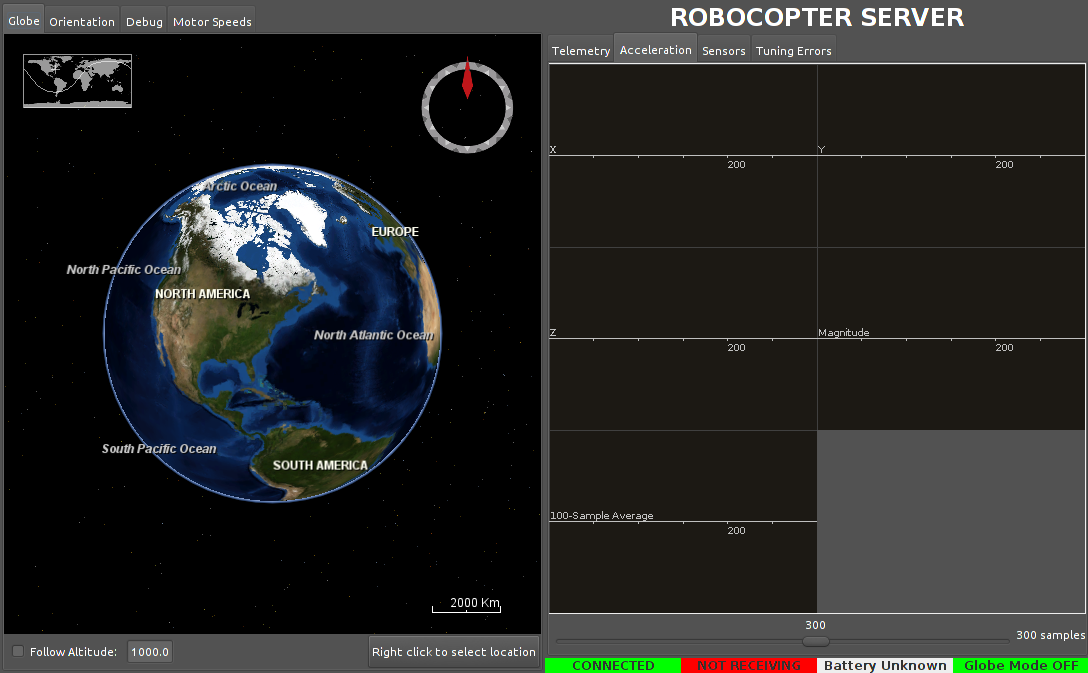
\includegraphics[scale=0.3]{figures/globe-screenshot}
  \caption{A screen capture of the chopper control software.}
  \label{fig:globe}
\end{figure}

The software is designed for two purposes: control and
telepresence. We have implemented a system which allows us to monitor
acceleration, orientation, temperature, location and even magnetic
flux. We also are streaming video from the helicopter to the server
software, which is displayed in the UI. We have a control subsystem
that allows us to control the helicopter from a mouse-based system, a
keyboard based system or a Microsoft XBOX controller. 

\subsection{Message Handling}
Sensor readings from the phone are transmitted to the server using
very simple strings, as is described in Section \ref{sec:msgs}. These
are received and placed into a message queue which handles all
subsequent processing. The various components of the UI and backend
are all programmed as plugins to this message queue handler. Each
plugin registers a list of prefixes with the message queue -- these
define the messages that that plugin is capable of processing. For
example, the orientation component handles only messages with the
prefix ``ORIENT'', while the PID tuning component handles anything
that starts with ``GUID'' or ``NAV'' (for guidance and navigation,
respectively). The appropriate messages then get passed onto these
components who handle the messages themselves.

The message handler receives a huge firehose of information, and only
about 10\% of the plugins need to respond to any given message. In
early implementations, every plugin received every message, which
meant that about 90\% of the work on each message was useless. In
instrumenting early builds using
VisualVM\footnote{http://openjdk.java.net/projects/visualvm/}, we
found that about 60\% of the processing done by the sever was trying
to handle each of the messages, and often the queue would fill faster
than it was emptying. The result was poor; there was a high latency
between sensor readings and display in the UI, and other components of
the server, such as the globe interface, always felt jerky because so
much processing power was devoted to message handling. Two fixes
improved this: the prefix-based handling (which cut down on processor
usage) and multithreaded plugins. Some of the plugins were blocking
the processing of later messages because the plugins were given new
messages synchronously -- switching to an asynchonous update mechanism
for some of the heavier plugins allowed us to decrease latency in
sensor readings and other easier-to-process messages.

\subsection{Telepresence}
The main thing we tried to accomplish in designing the UI was to make
it as easy to understand what the helicopter was doing as possible,
and be able to access all of the data the Android platform was capable
of giving us. We also wanted it to be easy to detect error conditions
at a glance for faster operator response to emergencies.

We eventually decided that, for many sensors, graphing them was the
most intuitive way to do this. To graph them, we rolled our own
graphic package (which was later released as SimpleGraph, a standalone
Java line graph library). For three, however, there were more
intuitive ways of displaying our data. For orientation, we used a 3D
representation of the helicopter that accurately mirrors the
orientation of the actual phone, which is easier to read than trying
to apply three rotations in your head. We used the
Java3D\footnote{https://java3d.dev.java.net/} game library for this,
which we chose because it was the most resource-efficient in our
testing. For location, we chose to mimic the Google Earth interface
and used NASA's World
Wind\footnote{http://worldwind.arc.nasa.gov/java/} mapping
software. This is an extraordinarily powerful library, and the only
one we could find of its kind. While poorly documented, the fact that
it was open source and very easy to use meant that we dropped this
into our UI quickly and seamlessly. The last visualization we used was
a very simple top-down view of the helicopter for the motor speeds, in
which each ``motor'' is given a color from red to green, denoting the
current speed of the motor.

\section{Hardware}
A list of parts used is supplied in Appendix \ref{tab:parts}.

\subsection{Design of the Chassis}
The chassis is the part whose design has fluctuated the most over the
process. While the software stack was fairly well-thought-out early
on, we wrote it to be hardware-independent. At first, the plan was to
use a kit chassis and buy our own components, as this would mean that
all of the components would be guaranteed to work together. However,
as time went on, we realized that the added cost of a robust chassis
was higher than the value we were getting out of it, and we decided to
build our own.

Using a 3D printer, we were able to print whatever plastic parts we
desired out of ABS plastic. ABS is a rigid and strong plastic -- it is
best known for being the raw form of a Lego brick -- and is very cheap
to buy in large quantities. Will owns a Makerbot that is capable of
printing objects up to 10cm by 10cm by 13cm, so it wasn't large enough
to build the entire helicopter in one go. Our design, therefore, had
to account for the fact that no individual custom-made part could be
larger than this.

\begin{figure}[htb]
  \centering
  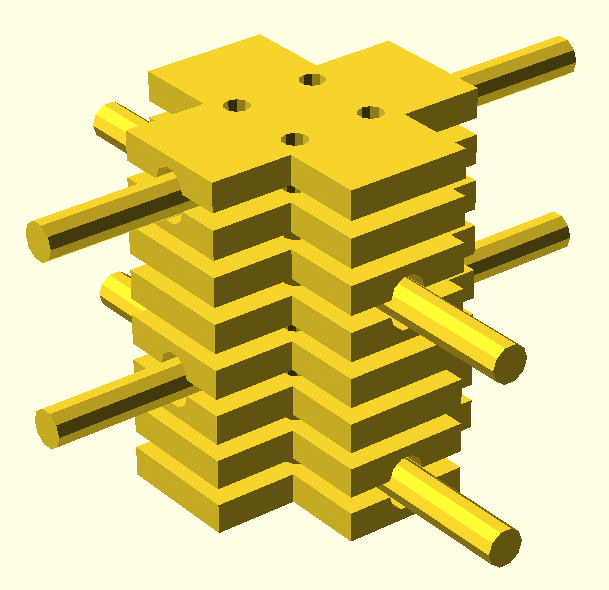
\includegraphics[scale=0.4]{figures/brock_assembly}
  \caption{(Brock) The center assembly upon which the electronics and
    Android device are mounted.}
  \label{fig:brock}
\end{figure}

\begin{figure}[htb]
  \centering
  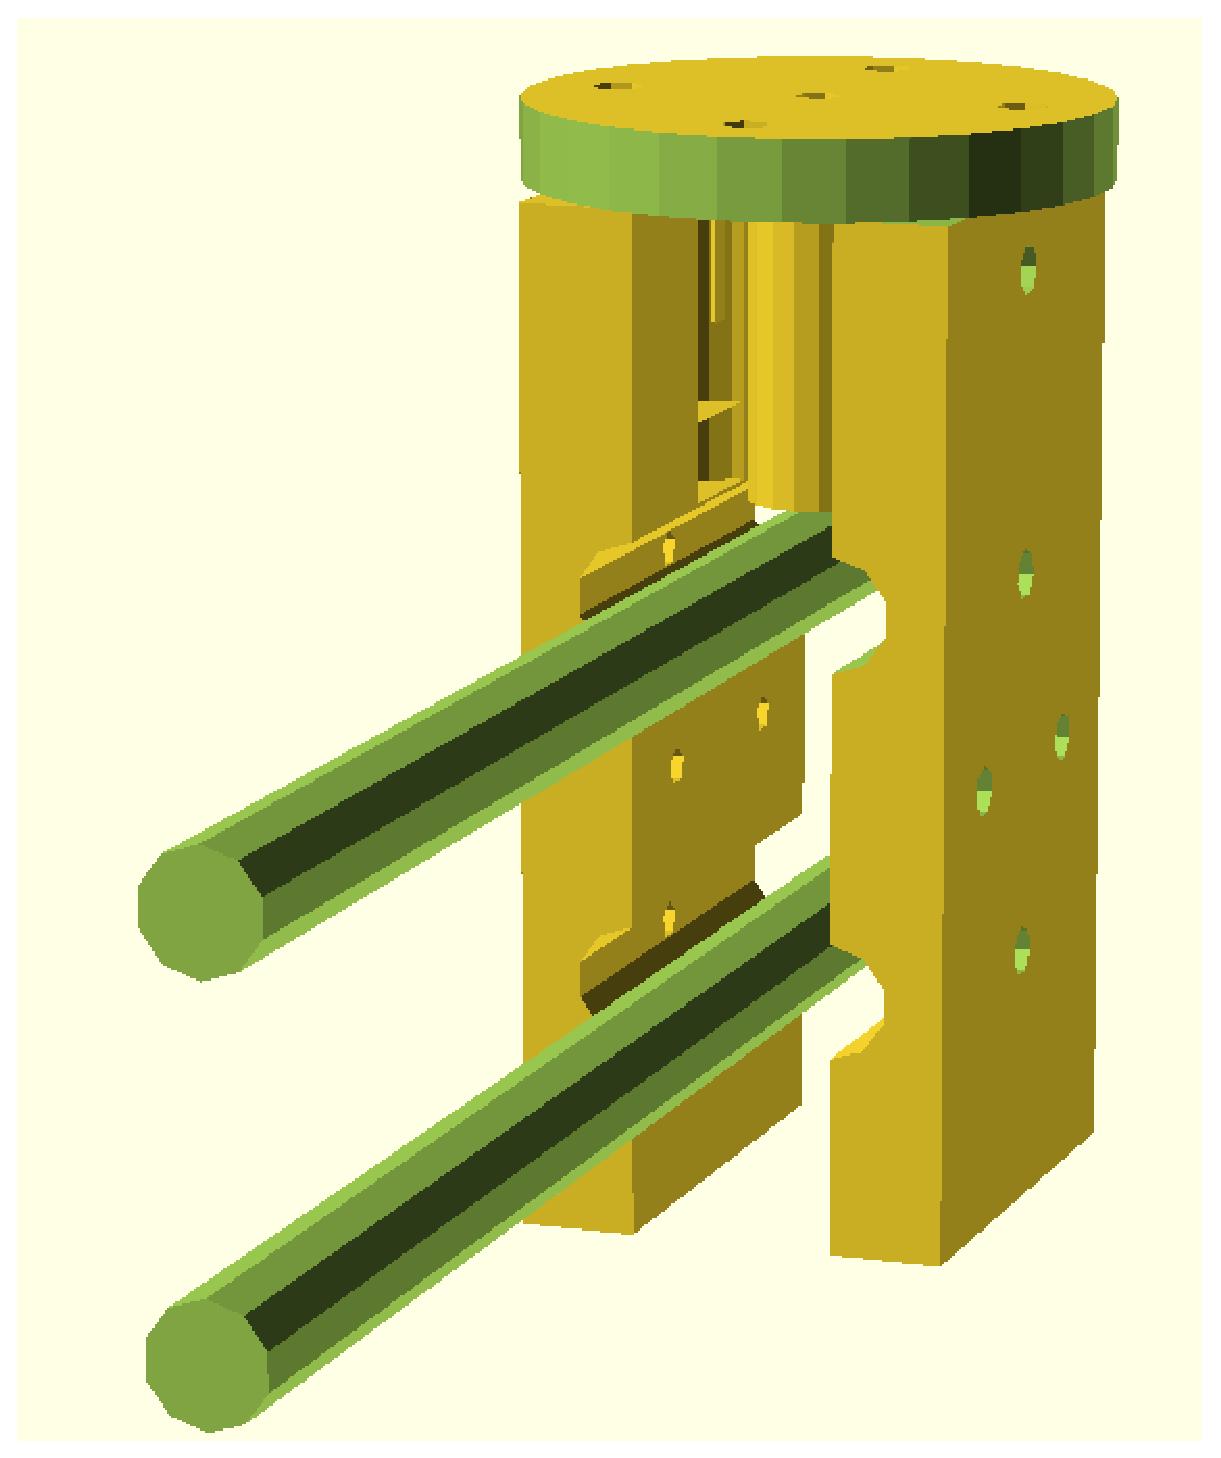
\includegraphics[scale=0.4]{figures/fred}
  \caption{(Fred) A motor mount on the end of a pipe.}
  \label{fig:fred}
\end{figure}

We opted for a design that is slightly different from most
commercially-available quadricopter designs for both pragmatic and
strength reasons. Our design features a large block in the middle made
of sandwiched layers, each of which holds a narrow-gauge brass pipe in
place. A rendering of this component can be seen in Figure
\ref{fig:brock}. These brass pipes extend 25 cm out either side of this
center block. On the end of each pipe is a motor unit, consisting of
two sandwiched ABS pieces that attach the motor to the pipe. This can
be seen in Figure \ref{fig:fred}.

Both the center layers (collectively called Brock) and the outer motor
mounting pieces (called Freds) require a stiff connection with the
brass pipes. However, we wanted to make this modular so we could
rebuild and redesign incrementally, and thus we didn't want to attach
the pipes directly to these pieces. Instead, we took a twofold
approach to ensuring the pipes would not slip. Firstly, we lined each
contact point between the model and the pipes with thin but
compressable foam, which is adhered to the plastic pieces. This foam
is both cheap and has a high coefficient of friction when in contact
with smooth surfaces, so it was perfect for this application. In
addition, we machined the pipes to have holes approximately 2.5 cm
from each end. The Fred pieces have holes placed so that a machine
screw can pass through Fred and the pipe, locking them together.

In order to create the requisite tension to hold the pipes in place in
Brock, we used four large machine screws through the center of the
piece. These provide the structural support for Brock. In addition,
the first and last layer of Brock each have eight mounting holes
with a captive nut locked in between the outer layer and next
layer. This allows us complete modularity in terms of hardware
attachments without ever having to reprint Brock -- all we must do is
make sure it is compatible with the mounting screws already built in,
and we can hotswap our hardware safely.

\subsection{Electronics Design}
In designing the electronics, we went for as much redundancy as
possible, and only used parts that had ratings at least 50\% over our
estimated needs. We estimated that the helicopter would have a weight
of approximately 1 kg (which ended up being a bit lower than the
actual weight) so each motor-propeller pair needed to be rated to
carry at minimum 500 grams. In addition, we wanted to be able to put
different payloads on the helicopter in the future (if we wanted to
add a video camera, for example) so we ended up going with
motor-propeller pairs that are capable of a very large range of
possible thrusts, from around 50 grams to about 1.5 kg per motor.

For our control hardware, we chose to use an Arduino because we had
experience coding for the Arduino software stack, and it provides many
libraries that are helpful for motor control and sensor
readings. While the sensor reading libraries will not be used in this
first iteration, in later iterations we plan on using rangefinding
sensors for landing and real-time distance map creation, so we wanted
to make sure we had the capability to hook that in to the existing
system.

We chose our other parts based on online reviews and price. One of our
goals was to keep this project as cheap as possible for two reasons;
firstly, we wanted to be able to pay for the thing, and secondly, we
were interested in seeing just how cheaply this could be done. In the
end, we managed to keep the cost low -- \$380 before tax and shipping,
for a per-person cost of only \$190.

We did make one fairly nonconventional decision in terms of
electronics design. While many designs use only one battery to power
the entire system, we chose instead to have four batteries -- one for
each motor. This has the disadvantage that we have to monitor four
battery capacities instead of one, the wiring is slightly more
complex, and the batteries can discharge at different rates. However,
having the four batteries has two distinct advantages: stability and
increased longetivity. The batteries are placed on the arms of the
helicopter, and the addition of the weight on these arms will help to
keep the helicopter more stable. It would be difficult to place a
single rectangular battery on our design without moving the
helicopter's center of gravity. Also, having all four batteries means
we can stay flying for longer, which is a clear advantage.

\subsection{Hardware Failure}
\label{sec:failure}
Before we even were able to take off, we had a dramatic hardware
failure that prevented us from being able to fly this semester. Each
motor requires a very specific input signal to rotate at the correct
rate. This is handled by devices called Brushless Electronic Speed
Controllers, or BESCs. These devices operate at extremely high
currents and temperatures, and thus have the potential to be extremely
dangerous when they malfunction. Because of this danger, and because
of the fact that if one were to fail while we were flying, the
helicopter will no doubt be broken or destroyed, we tested them
thoroughly before attaching them to the chassis of the helicopter.

All of them performed admirably with the exception of one, which had a
faulty chip inside. When plugged in, it smoked profusely. Assuming
that there was a short somewhere inside, we opened it up to take a
look, and plugged it back in to see if we could see where the smoke
was coming from (also, we grabbed a fire extinguisher and put it on a
flameproof mat). As soon as it was plugged in, one of the
microcontrollers burst into flame, which, while dramatic and pretty
cool, suggested that perhaps that BESC shouldn't be used on our
helicopter. Two weeks later, and we are still waiting for the
replacement part from the retailer -- as soon as we receive this part
in the mail, we'll be able to start testing and flying.

\section{Communication}
Communication is composed of two main components:‭ ‬telemetry and
commands/data.‭ ‬Each is relayed on separate ports,‭ ‬since commands must
be relayed as synchronously as possible and telemetry will be
asynchronous.

\subsection{Telemetry}
The telemetry modules continuously run the Android's preview
functionality,‭ ‬at‭ ‬5fps.‭  ‬Each frame is saved to a buffer as it is
available,‭ ‬overwriting the previous frame.‭  ‬When the Android has
finished sending one frame to the control server,‭ ‬it immediately
copies the buffer and starts sending the frame.‭  ‬The result is real
time telepresence,‭ ‬at approximately‭ ‬1-2‭ ‬fps and a lag of‭ ‬1‭ ‬frame.

\subsection{Commands and Data}
Commands and data are relayed in the form of strings over standard
Java sockets.‭ ‬When the connection is lost,‭ ‬the Android immediately
tries to reconnect,‭ ‬continuing to do so indefinitely.‭ ‬While the
connection is lost,‭ ‬autopilot is enabled and the‭ “‬communication lost‭”
‬pre-programmed instruction set is engaged.

\subsection{Message Formats}
\label{sec:msgs}
‏Messages between the Android and the control server are sent as
strings,‭ ‬delimited by colons.‭ ‬The strings from the control
server―commands―contain the instruction itself,‭ ‬prefixed by a sequence
of meta-data describing the instruction.‭ ‬Similarly,‭ ‬data from the
Android contain not just the data,‭ ‬but also a prefix tag describing
the data.‭ ‬This enables somewhat efficient analysis on each end:‭
‬messages can be routed only to those components that are registered to
process a given prefix tag.  Messages are not transmitted directly
between the Android and the control server.‭ ‬Instead,‭ ‬they are routed
through a separate,‭ ‬dedicated broker server.‭ ‬This enables the control
server itself to operate easily from different IP addresses,‭ ‬and hence
from various locations. It also allows for easy logging and playback
of sessions -- the broker server logs all data and commands, and can
replay a session so we can analyze what happened.

\newpage
\appendix
\section{Parts and Prices}
\label{tab:parts}
\begin{tabular}{llll}
  \textbf{Item} & \textbf{Supplier}
  & \textbf{Quantity} & \textbf{Price} \\

  Chassis Hardware & McMaster-Carr & N/A & \$32.60 \\
  Turnigy 2217 Brushless Motors & HobbyKing & 4 & \$14.04 \\
  Counterforce Propeller Pair & NG Hobbies & 5 & \$6.95 \\
  Arduino Microcontroller & SparkFun & 1 & \$29.95 \\
  Turnigy 15 Amp ESC Controller & HobbyKing & 4 & \$10.58 \\
  BlueSmirf Gold Bluetooth Modem & SparkFun & 1 & \$64.95 \\
  Turnigy 2200mAh 3S LiPoly Battery & HobbyKing & 5 & \$11.96 \\
  Arduino ProtoShield Layout PCB & SparkFun & 1 & \$16.95 \\
  HobbyKing Fast Battery Charger & HobbyKing & 1 & \$39.99 \\
\end{tabular}

\section{Code Repository}
A single github repository is used for version control of the server,
client and broker, as well as this essay.

http://github.com/haldean/droidcopter

\end{document}